\documentclass[letterpaper,10pt]{article}

\usepackage{enumitem}
\usepackage{titling}
\usepackage{listings}
\usepackage{url}
\usepackage{hyperref}
\usepackage{setspace}
\usepackage{subfig}
\usepackage{sectsty}
\usepackage{pdfpages}
\usepackage{colortbl}
\usepackage{multirow}
\usepackage{multicol}
\usepackage{relsize}
\usepackage{amsmath}
\usepackage{wasysym}
\usepackage{fancyvrb}
\usepackage[yyyymmdd]{datetime}
\usepackage{amsmath,amssymb,amsthm,graphicx,xspace}
\usepackage[titlenotnumbered,noend,noline]{algorithm2e}
\usepackage[compact]{titlesec}
\usepackage{XCharter}
\usepackage[T1]{fontenc}
\usepackage[scaled]{beramono}
\usepackage[normalem]{ulem}
\usepackage{booktabs}
\usepackage{tikz}
\usetikzlibrary{arrows,automata,shapes,trees,matrix,chains,scopes,positioning,calc}
\tikzstyle{block} = [rectangle, draw, fill=blue!20,
text width=2.5em, text centered, rounded corners, minimum height=2em]
\tikzstyle{bw} = [rectangle, draw, fill=blue!20,
text width=4em, text centered, rounded corners, minimum height=2em]

\definecolor{namerow}{cmyk}{.40,.40,.40,.40}
\definecolor{namecol}{cmyk}{.40,.40,.40,.40}
\renewcommand{\dateseparator}{-}

\let\LaTeXtitle\title
\renewcommand{\title}[1]{\LaTeXtitle{\textsf{#1}}}

\lstset{basicstyle=\footnotesize\ttfamily,breaklines=true}

\newcommand{\handout}[5]{
	\noindent
	\begin{center}
		\framebox{
			\vbox{
				\hbox to 5.78in { {\bf ECE 350: Real-Time Operating Systems } \hfill #2 }
				\vspace{4mm}
				\hbox to 5.78in { {\Large \hfill #4  \hfill} }
				\vspace{2mm}
				\hbox to 5.78in { {\em #3 \hfill \today} }
			}
		}
	\end{center}
	\vspace*{4mm}
}

\newcommand{\lecture}[3]{\handout{#1}{#2}{#3}{Lecture#1}}
\newcommand{\tuple}[1]{\ensuremath{\left\langle #1 \right\rangle}\xspace}

\newcommand{\Rplus}{\protect\hspace{-.1em}\protect\raisebox{.35ex}{\smaller{\smaller\textbf{+}}}}
\newcommand{\Cpp}{\mbox{C\Rplus\Rplus}\xspace}


\addtolength{\oddsidemargin}{-1.000in}
\addtolength{\evensidemargin}{-0.500in}
\addtolength{\textwidth}{2.0in}
\addtolength{\topmargin}{-1.000in}
\addtolength{\textheight}{1.75in}
\addtolength{\parskip}{\baselineskip}
\setlength{\parindent}{0in}
\renewcommand{\baselinestretch}{1.5}
\newcommand{\term}{Spring 2023}
\newcommand{\termnumeric}{1235}

\singlespace


\begin{document}

\lecture{ 11 --- Virtual Memory II }{\term}{Jeff Zarnett}

\section*{Virtual Memory, Continued}

We will continue with our discussion of virtual memory by looking at a few advanced considerations in virtual memory.

\subsection*{Memory-Mapped Files}
When we talked about inter-process communication in a previous course, one option that we covered was based around memory-mapped files. Now we can actually talk about how it works.

It should not be surprising, given what we know so far, that the basic premise is that disk blocks for the file are mapped to memory and if a chunk of the file is referenced that is not in memory, it is treated as if it is a normal page fault and a page-sized piece of the file is brought into memory~\cite{osc}. In this regard it is then expected that other accesses are just memory reads and writes on the data in memory without going to disk. When the file is closed, then the data is written back to disk in its modified format. 

In the one-process-using-it scenario, we don't have to worry so much about synchronizing changes, but in the inter-process communication version it was important to make sure that we chose to synchronize the file because changes might not be visible immediately. If two or more processes have the same file in memory at a time, the memory-mapped file can in the virtual address space for the two different processes. But remember, we only go and fetch a block of the file for this process if we need it, so some explicit synchronization is needed to be certain that the data is the same for everyone.

\subsection*{Arbitrary Addresses: Memory-Mapped I/O}
Another advanced consideration for I/O when we think of memory is the need for memory-mapped I/O -- to communicate with a certain hardware device, an area of memory is mapped to the I/O device's memory. This means that although it looks like an ordinary memory read or write to main memory, in reality it might be going over the bus to a totally different device. This simplifies some operations and implementations, because communicating with the device works exactly the same way as communicating with memory -- nothing special is needed.  Part of the reason behind treating everything like a file in UNIX is to simplify the operations; something similar applies here.

This contrasts with the older-style \textit{port-mapped} I/O where there are different CPU instructions and separate registers used to communicate with the device. It's not that this does not work, but it's just more difficult to work with.

\subsection*{Allocation of Frames}
In a simple system where we do not do anything advanced, if there are $n$ frames free in the system, we will demand page all of them. So the initial state is that all frames are empty, and as needed, pages are read into those frames. Once all $n$ frames are filled with pages, page $n+1$ must replace a page already in a frame (because there is no more space). When a process terminates, all its frames are marked as free. In theory, one process could fill all the frames in the system. This is as simple as it can be; from there we can build on it.

We might reserve a few pages to be free at all times for performance considerations. When we want to move a page into a frame, if all of the frames are full, we select a victim and write that victim out to disk if necessary. If we keep a few frames free, the newly-read page can be read into one of the free frames, and we can write the old page out to disk at a convenient time. The read does not need to wait for the write (flush of the old page) and therefore the user process gets to continue a bit sooner than it otherwise would.

Assuming, as we did with cache, that we might want to allocate different numbers of frames to different processes (and not necessarily let one run wild), we are constrained in the number of pages we can allocate. The maximum number of frames a process could have is the maximum number of frames in the system (obviously), but the minimum is more interesting.

The motivation behind allocating at least a minimum number of frames is ostensibly performance. As long as our page replacement algorithm is sane (i.e., not FIFO), adding more frames reduces the page fault rate. As we demonstrated earlier, a page fault is a huge performance decrease. 

The absolute minimum number of frames is determined by the architecture of the system. Imagine a machine where a memory reference instruction may contain one memory address. In the worst case, the instruction and the address are in different pages, so we will need two frames to be able to complete this instruction. If the max frames for this process were 1, the instruction could never be completed. 

Another possible thing that limits the number of frames that we can move around is the need to lock pages in memory. One possible cause of this locking is an I/O operation: if the I/O has been handed off to a DMA controller, the DMA has a source and destination address and one of those may be a specific memory location and we cannot move those pages to different frames or swap them out~\cite{osc}. When the I/O operation is started, lock the relevant frame or frames, and they are ineligible for replacement while locked; when the operation is complete, then unlock it/them. Frames is plural because it is possible that the data, even if small, crosses at least one page boundary. We could avoid the need for locking if, however, data reads and writes do not take place in user-level process memory and instead the data is copied to/from some kernel buffers.

Assuming we do not allocate every process the minimum or maximum, there are a few allocation algorithms we might follow. We already got a glimpse at this when we talked about local vs. global cache replacement.

If there are $m$ frames in the system and the operating system reserves $k$ of them for its own use, there are $m-k$ frames available for processes.

\paragraph{Equal Allocation.}  If there are $n$ processes in the system, if we allocate them equally, each process gets $(m-k)/n$ frames. If this division produces a remainder, the leftover frames can be kept as a pool of free frames for performance purposes as above. There is an obvious flaw in this plan: why does a text editing program get the same amount of frames as a web browser and the same amount of frames as a game (which tends to be VERY demanding on memory).

\paragraph{Proportional Allocation.} So how about proportional allocation: each process should get a share of the frames based on its needs. The strategy suggested in~\cite{osc} to do frame allocation runs something like this. Let the virtual memory size of a process $p_{i}$ be defined as $s_{i}$. Thus $S = \Sigma s_{i}$. If the total number of frames in the system is, once again, $m$, and the operating system reserves $k$ for itself, then we allocate $a_{i}$ frames to a process $p_{i}$ according to the following formula: $a_{i} = s_{i} / S \times (m - k)$.

This value of $a_{i}$ is only an estimate. It may not divide evenly, and we can only allocate an integer number of frames to each process.  So we will have to raise or lower $a_{i}$ a bit to make it an integer. If $a_{i}$ is below the minimum number of frames, then it needs to get bumped up to that minimum. We also must respect the limits of the system: the sum of all $a_{i}$ values may not exceed the total frames of memory (minus the OS reserve), so a few of the larger processes may need to have their allocations nudged down.

Note that with proportional allocation, as with equal allocation, there is no regard given to the priorities of the processes. Normally, we would want to give more frames to higher priority processes so their page fault rates are lower and they can therefore execute more quickly. So we could modify the $a_{i}$ values according to process priority, as well~\cite{osc}. The subject of priority is something we have not yet examined much yet, but will do so soon when we get to talking about scheduling; the next major topic. But, first, let's finish what we are doing with memory.


\subsection*{Thrashing}
Thrashing received a little bit of mention in the introduction to virtual memory, but it deserves some further consideration. The quick definition of thrashing still applies: the operating system is spending so much time moving pages into and out of memory that no useful work gets done. Aside from intentionally depriving the system of RAM (as in the NeXTStep scenario), how can we get into this state, and how can we get out of it?

Let's consider a simple example from~\cite{osc}. In simple operating systems, the logic that controlled how many processes to run at a time would rely just on the CPU utilization. If CPU utilization is low, the CPU needs more work to do! Assign it more work by starting or bringing more processes into memory. The global page replacement policy is used here, so when a process gets a page fault, it takes a frame from another process. Under most circumstances, this works just fine.

This situation is not obviously wrong until one process starts to have a lot of page faults. This is not unreasonable; a compiler might be finished with reading and parsing the input files and moving to generation of binary code, for example, which requires a whole bunch of new instructions pages, plus the pages for the output. When this process does so, it starts taking pages from other processes. The victim processes need the pages they had, so when they get a turn to run, they too start generating page faults. So more and more requests are queued up for memory writes and reads, so the CPU is not very busy. Here's the fatal mistake: seeing that the CPU is not very busy, the OS schedules \textbf{more} programs to run.  

A new process getting started will need at least the minimum number of pages to get started. These have to come from somewhere, so they will necessarily come from the pages currently belonging to other processes. This causes more page faults and more time spent paging and lower CPU utilization... prompting the OS to start more processes. No more work is getting done, because the system spends all its time moving pages into and out of memory, thrashing all around, acting like a maniac\footnote{Whiplash! ... If this joke means nothing to you, it's also because I'm old.}.

\begin{center}
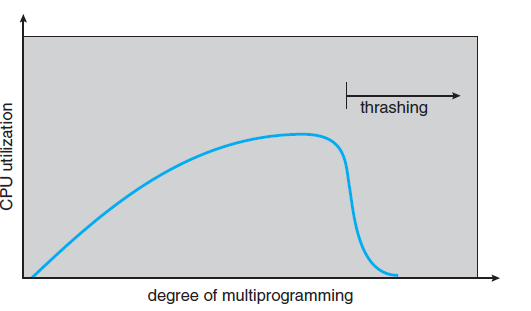
\includegraphics[width=0.5\textwidth]{images/thrashing.png}\\
Thrashing~\cite{osc}.
\end{center}

The solution is simple, actually; to increase CPU utilization we need to stop the thrashing which means we need fewer programs in memory at a time. What this really tells us is that CPU usage alone is not a sufficient indicator of whether more or fewer processes need to be running right now. It also matters \textit{why} the CPU utilization is low. Another reason that might cause low CPU usage is, as you may recall, deadlock. 

 What if we stop using a global replacement policy and instead force local replacement? This limits some of the damage; if Process $P_{1}$ is thrashing,it cannot steal pages from $P_{2}$ and we do not get a cascade where all processes are constantly fighting over who has how many pages. But, if $P_{1}$ is spending all its time paging to and from disk, any other process that wants to use the disk (whether to swap or to interact with files) is going to have to spend more time waiting for the disk to be free.  
 
We could decide whether we need to start or suspend programs not just based on CPU usage, but also on the number of page faults that occur in a given period of time. If there are too many page faults, it indicates we have too much going on. That is a reactive solution, however, and might only engage after a fair amount of time and effort has been wasted in thrashing. It would be better to be proactive and deal with this before thrashing has started.
 
As is typical, a bit of clairvoyance would help here: how many pages is the process going to need and when will it need them? Unfortunately, there is no good way to know or to figure this out. So we will have to rely on (educated) guessing. You may hate the idea of guessing. As a general engineering practice, ``let's do an experiment and find out'' is good, provided you can analyze the result and if things go horribly wrong, no damage is done. Those last conditions make it kind of infeasible to do medical experiments just to see what would happen, or for NASA to play around with satellites in orbit. So in those cases, a simulation is probably the better approach. Even so, sometimes we don't have (or can't get) the data we need and we will therefore need to ``make our best guess''. But we are digressing.

What do we know about process memory accesses? They tend to obey the principle of locality, both temporal and spatial. Recall this from the discussion about caching. We could think of different parts of the program as different localities, as if they were areas on a map. And localities may overlap sometimes. So what we would like to do, then, is give a process enough frames for its locality. If we do so, it can operate in this little area without encountering (too many) page faults. If we give insufficient pages, the process will be thrashing. Eventually it will leave the locality and that will result in some more page faults, but this is generally unavoidable~\cite{osc}.  

Before coming up with a solution that relies on locality, it is a good idea to check that the principle of locality holds. Fortunately we do not have to verify this for ourselves; someone else has already done so:

\begin{center}
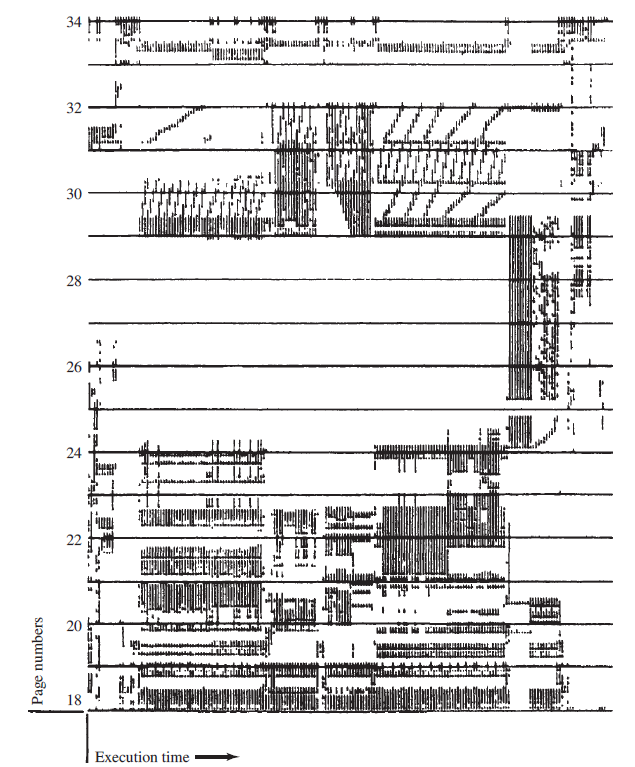
\includegraphics[width=0.75\textwidth]{images/locality.png}\\
Graph showing the locality of memory accesses -- it is real!~\cite{locality}.
\end{center}

The take-away from this graph is that yes, locality is real. Given that, we can now move on and use it.


\subsection*{The Working-Set Model}

A potential solution is the working-set model as described in~\cite{osc}. We retain the last $n$ pages in memory as they represent the locale of the program. Assuming that most memory accesses are local, the most recent $n$ pages will be the most frequently used. In the textbook descriptions, this $n$ is usually called $\Delta$,the working set window. Pages that have been recently used are in the working set. If a page has not been accessed recently, it will drop out of the working set after $\Delta$ time units since its last reference. 

Suppose the window is defined as being ten accesses. Any page that was accessed in the last ten requests will then be considered part of the working set. If the next ten memory accesses are all in page $k$, then after those further ten accesses, the working set will contain only $k$. So the size of the working set will change over time and can be anywhere from 1 to $\Delta$ pages.

If $\Delta$ is too small, the working set will not encompass the entire locale. If it is too large, it will cover multiple locales. Underestimating the size of the locale is bad, because it will mean more page faults being caused. Overestimating is also bad, because it means fewer processes will be allowed to run.

If the working set of every process is summed up, we will get the total number of frames each process would ``like'' to have. If this sum exceeds the $(m-k)$ available frames in the system, at least one process is going to be unhappy because it does not have as many frames as it will need. And like unhappy workers who go on strike, unhappy process start thrashing.

Once a value of $\Delta$ is determined, the OS will monitor the working set of each process and use that to figure out if the system is currently overloaded. If it is, the OS will pick a victim and suspend it to prevent thrashing. If the system is underloaded (frame supply exceeds demand), more processes can be started to run.

Now we should examine how this solution works. The page fault rate of a process tends to vary over time. At the beginning, there will be a bunch of page faults as the program starts up. Then once established in its first locale, the rate will drop. When it come time to move to a new locale, the page fault rate rises until the program is ``settled'' in that new locale. See the graphic below:

\begin{center}
	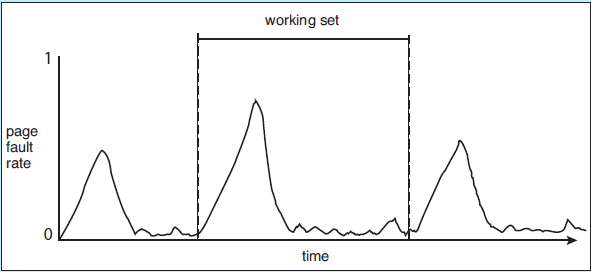
\includegraphics[width=0.5\textwidth]{images/workingset.png}
\end{center}

Here's an analogy. Imagine that you have moved to a new city for a co-op term. When you have just moved, you will frequently rely on Google Maps (or whatever other map program you like... or even, dare I say it, the paper ones?!) to find what you are looking for and how to get there. You need to buy groceries, so you ask Google for directions to the nearest grocery store of choice. Once you've been there, you know the way so you don't have to ask again. Not knowing where the grocery store is equals a page fault, and asking Google is like asking the operating system to bring in that page from disk. Once you know the way to the grocery store, it is part of your working set and you do not have to ask again... until your next co-op term when you move somewhere else.

\bibliographystyle{alphaurl}
\bibliography{350}


\end{document}
